\section{Receptor UART (\texttt{uart\_rx})}

El receptor es responsable de transformar la señal serie \texttt{rx} en un byte paralelo y anunciar cuándo el dato está listo. Emplea \textbf{oversampling} a $16\times$ y una máquina de estados finitos (FSM) con temporización por ticks.

\subsection{Trama y convenciones}
La línea \texttt{rx} permanece en nivel alto en reposo. Cada trama se compone de:
\begin{itemize}
    \item \textbf{Start}: 1 bit en nivel bajo.
    \item \textbf{Datos}: \(\texttt{DBIT}=8\) bits, orden \textit{LSB first}.
    \item \textbf{Stop}: 1, 1.5 o 2 bits en alto, parametrizados por \(\texttt{SB\_TICK}\in\{16,24,32\}\).
\end{itemize}

\subsection{Señales y contadores internos}
\begin{itemize}
    \item \texttt{sample\_tick}: pulso de temporización a \(16\times\) la tasa de baudios.
    \item \texttt{tick\_count}: cuenta los ticks dentro del bit (0..15 para datos).
    \item \texttt{bit\_count}: cuenta cuántos bits de datos se han muestreado (0..DBIT-1).
    \item \texttt{rx\_shift\_reg}: registro de desplazamiento donde se van incorporando los bits recibidos.
    \item \texttt{rx\_done\_tick}: pulso de un ciclo de \texttt{clk} que indica “byte listo”.
\end{itemize}

\subsection{Máquina de estados y flujo temporal}
La FSM consta de cuatro estados: \textbf{IDLE}, \textbf{START}, \textbf{DATA} y \textbf{STOP}. El funcionamiento se describe paso a paso a continuación y se ilustra en la Figura~\ref{fig:uart-rx-fsm}.

\paragraph{1) IDLE (espera de start)}  
La línea \texttt{rx} está alta. Al detectarse un nivel bajo (\emph{start bit}), se pasa a \textbf{START} y se reinicia \texttt{tick\_count}.

\paragraph{2) START (centrado de muestreo)}  
Con cada \texttt{sample\_tick} se incrementa \texttt{tick\_count}. Al alcanzar \(\texttt{tick\_count}=7\) (8 ticks desde el flanco), se considera que estamos en el \textbf{centro} del start. Entonces:
\begin{enumerate}
    \item Se pone \texttt{tick\_count} en 0 para comenzar a cronometrar el primer bit de datos.
    \item Se pone \texttt{bit\_count} en 0.
    \item Se transita a \textbf{DATA}.
\end{enumerate}

\paragraph{3) DATA (muestreo de 8 bits)}  
Cada vez que \(\texttt{tick\_count}=15\) y llega \texttt{sample\_tick}, se toma la muestra del bit (centro del bit) y se la introduce al MSB del \texttt{rx\_shift\_reg} desplazando a la derecha. Esto, repetido 8 veces con \textit{LSB first}, deja el registro en orden natural \([b7\ldots b0]\). Tras cada muestreo:
\begin{itemize}
    \item \texttt{tick\_count} se reinicia a 0.
    \item \texttt{bit\_count} se incrementa.  
          Si \(\texttt{bit\_count}= \texttt{DBIT}-1\), se pasa a \textbf{STOP}.
\end{itemize}

\paragraph{4) STOP (validación y fin de trama)}  
Se esperan \(\texttt{SB\_TICK}\) ticks (por defecto 16 para 1 bit de stop). Al cumplirse:
\begin{itemize}
    \item Se genera un pulso \texttt{rx\_done\_tick} indicando que el byte en \texttt{dout} es válido.
    \item Se vuelve a \textbf{IDLE}.
\end{itemize}

\begin{figure}[H]
    \centering
    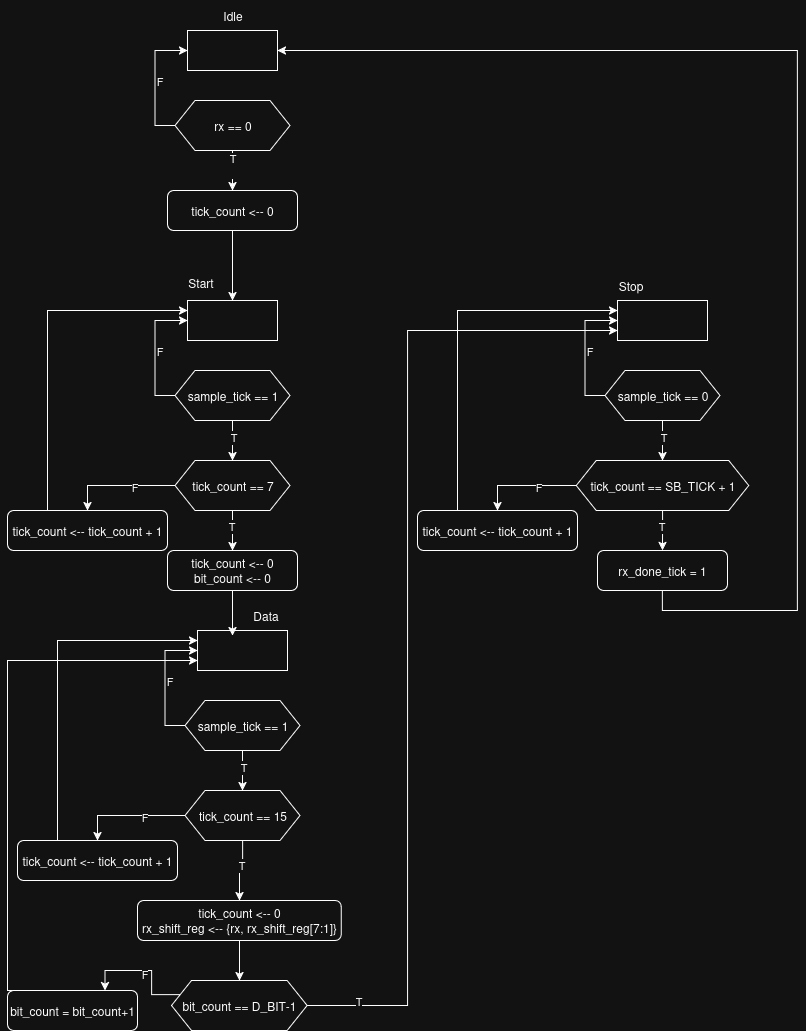
\includegraphics[width=0.95\textwidth]{img/diagramaReceiverUART.png}
    \caption{Diagrama de flujo de la FSM del receptor UART con oversampling a \(16\times\).}
    \label{fig:uart-rx-fsm}
\end{figure}

\subsection{Cronometría: instantes de muestreo}
Tras detectar el start, el primer muestreo útil ocurre \(8\) ticks después (centro del start) y luego cada \(16\) ticks para cada bit de datos. El tiempo total entre el flanco de start y el anuncio del byte listo es:
\[
N_{\text{ticks}} = 8 + 16\cdot \texttt{DBIT} + \texttt{SB\_TICK}
\]
Para \(\texttt{DBIT}=8\) y \(\texttt{SB\_TICK}=16\): \(N_{\text{ticks}}=152\).  
Como \(T_{\text{tick}}=\tfrac{1}{16\cdot BAUD\_RATE}\), el retardo es aproximadamente \(152 \cdot T_{\text{tick}} \approx 0{,}99\,\text{ms}\) a \(9600\,\text{bps}\), coherente con una trama de 10 bits (\(\sim 1{,}04\,\text{ms}\)), considerando que el muestreo se inicia en el centro del start.

\subsection{Parámetros y salidas}
\begin{itemize}
    \item \textbf{\texttt{DBIT}}: número de bits de datos (8 en este diseño).
    \item \textbf{\texttt{SB\_TICK}}: cantidad de ticks de stop (16, 24 o 32 $\Rightarrow$ 1, 1.5 o 2 bits).
    \item \textbf{\texttt{dout}}: byte paralelo reconstruido a partir de \texttt{rx\_shift\_reg}.
    \item \textbf{\texttt{rx\_done\_tick}}: pulso de 1 ciclo de \texttt{clk} indicando dato válido.
\end{itemize}

\subsection{Notas de diseño y posibles mejoras}
\begin{itemize}
    \item \textbf{Sincronización del pin \texttt{rx}}: al ser asíncrono respecto de \texttt{clk}, es recomendable anteponer un \emph{doble flip-flop} de sincronización para mitigar metastabilidad.
    \item \textbf{Detección de error de trama}: durante \textbf{STOP} verificar que \texttt{rx} esté alto; si no, reportar \emph{framing error}.
\end{itemize}
